\chapter{Arkitektur}
I dette afsnit vil der blive beskrevet den overordnede arkitektur for Rambøll Tilsyn.

På Figur \ref{fig:Domain} ses domæne modellen for Rambøll Tilsyn. Her ses, hvilke dele systemet indeholder og hvilken relation de har til hinanden.
For den fulde arkitektur henvises til Arkitektur og Design dokumentationens Afsnit \ref{Design-sec:Arkitektur} Arkitektur.

\begin{figure}[H] % (alternativt [H])
	\centering
	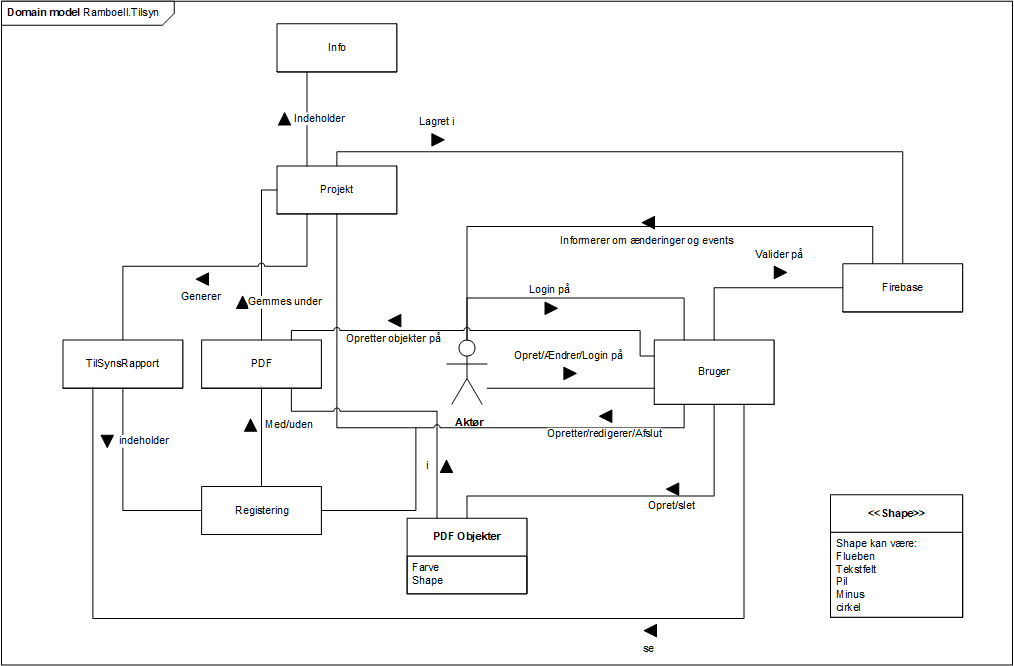
\includegraphics[height=13cm, width=17cm]{Arkitektur/Domainmodel}
	\caption{Domænemodel for Rambøll Tilsyn.}
	\label{fig:Domain}
\end{figure}

\clearpage

På Figur \ref{fig:KlasseDiagram} ses der en klassediagram over Rambøll TilSyn. Klassediagrammet viser klasserne i Rambøll Tilsyn og hvilke relationer disse har.
\begin{figure}[H] % (alternativt [H])
	\centering
	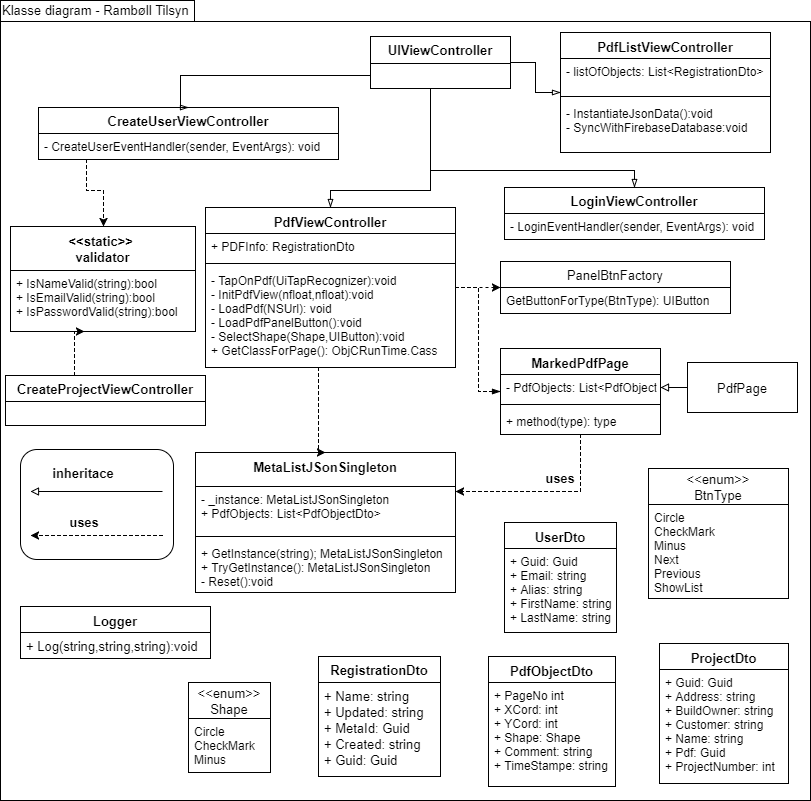
\includegraphics[height=13cm, width=17cm]{Arkitektur/KlasseDiagram}
	\caption{Klassediagram for Rambøll Tilsyn.}
	\label{fig:KlasseDiagram}
\end{figure}


Alle ViewControllers er nedarvet fra UIViewController\cite{UIViewController}. UIViewController er en klasse, der stammer fra Xamarin.iOS frameworket. \\
Klassen UITableViewControllers formål er at vise en liste af data, som man selv har implementeret. \\
Logger klassen bruger Firebase Analytics\cite{FirebaseAnalytic} for at logge events fra applikationen. Dette gør, at man kan bruge fejlmeddelelserne fra Analytics til at fortælle brugeren, hvad der er sket af fejl.  
